\documentclass[11pt,a4paper]{article}

% ── Packages ──────────────────────────────────────────────────────────────────
\usepackage[utf8]{inputenc}
\usepackage[T1]{fontenc}
\usepackage{lmodern}
\usepackage[margin=2.5cm]{geometry}
\usepackage{amsmath,amssymb}
\usepackage{booktabs}
\usepackage{enumitem}
\usepackage{graphicx}
\usepackage{xcolor}
\usepackage{hyperref}
\usepackage{tikz}
\usetikzlibrary{positioning, arrows.meta, fit, calc, shapes.geometric}
\usepackage{float}
\usepackage{caption}
\usepackage{subcaption}
\usepackage{algorithm}
\usepackage{algpseudocode}
\usepackage{tabularx}
\usepackage{fancyhdr}

% ── Colors ────────────────────────────────────────────────────────────────────
\definecolor{darkblue}{HTML}{1B3A5C}
\definecolor{accentblue}{HTML}{2E86C1}
\definecolor{highlightred}{HTML}{E74C3C}
\definecolor{lightgray}{HTML}{F2F2F2}

\hypersetup{
    colorlinks=true,
    linkcolor=darkblue,
    urlcolor=accentblue,
    citecolor=darkblue,
}

% ── Header / Footer ──────────────────────────────────────────────────────────
\pagestyle{fancy}
\fancyhf{}
\fancyhead[L]{\small\textcolor{darkblue}{AISA Hackathon -- Surrogate Modeling}}
\fancyhead[R]{\small\textcolor{darkblue}{\thepage}}
\renewcommand{\headrulewidth}{0.4pt}

% ── Title ─────────────────────────────────────────────────────────────────────
\title{%
    \textcolor{darkblue}{\textbf{Multi-Task Surrogate Models for\\
    Mechanical MNIST Cahn--Hilliard}}\\[0.5em]
    \large Model Architecture and Training Documentation
}
\author{AISA Hackathon}
\date{\today}

% ══════════════════════════════════════════════════════════════════════════════
\begin{document}
\maketitle
\thispagestyle{fancy}

\begin{abstract}
This document provides a detailed description of two neural network surrogate
models developed for the Mechanical MNIST Cahn--Hilliard dataset: a
\textbf{Multi-Task U-Net} (${\sim}8.1$M parameters) and a
\textbf{Multi-Task Fourier Neural Operator} (${\sim}2.7$M parameters).
Both models simultaneously predict displacement fields, strain energy, and
reaction forces from binary microstructure images, replacing expensive finite
element simulations with fast neural network inference.
\end{abstract}

\tableofcontents
\newpage

% ══════════════════════════════════════════════════════════════════════════════
\section{Problem Description}
\label{sec:problem}

\subsection{Dataset Overview}

The \textbf{Mechanical MNIST Cahn--Hilliard} dataset contains 104,813 samples
of binary heterogeneous microstructures generated via the Cahn--Hilliard
equation. Each sample is paired with finite element analysis (FEA) simulation
results computed using FEniCS.

\begin{table}[H]
\centering
\caption{Dataset composition.}
\label{tab:dataset}
\begin{tabular}{@{}lrr@{}}
\toprule
\textbf{Case} & \textbf{Samples} & \textbf{Image IDs} \\
\midrule
Case 1 & 37,523 & 1 -- 37,523 \\
Case 2 & 37,680 & 37,524 -- 75,203 \\
Case 3 & 29,610 & 75,204 -- 104,813 \\
\midrule
\textbf{Total} & \textbf{104,813} & \\
\bottomrule
\end{tabular}
\end{table}

The physical simulation applies \textbf{equibiaxial loading} to a binary
Neo-Hookean material at seven displacement levels:
\[
    d \in \{0.0,\; 0.001,\; 0.1,\; 0.2,\; 0.3,\; 0.4,\; 0.5\}.
\]

\subsection{Prediction Targets}

Both models are trained as \textbf{multi-task} learners with three output heads:

\begin{enumerate}[leftmargin=2em]
    \item \textbf{Displacement fields} --
          Two spatial fields $u_x, u_y \in \mathbb{R}^{64 \times 64}$
          representing the $x$- and $y$-direction displacements at $d = 0.5$.
          Output shape: $(B, 2, 64, 64)$.

    \item \textbf{Strain energy} --
          Seven scalar values, one per displacement level.
          Output shape: $(B, 7)$.

    \item \textbf{Reaction forces} --
          Twenty-eight scalar values (4 boundaries $\times$ 7 displacement levels).
          Boundaries: left-$x$, right-$x$, bottom-$y$, top-$y$.
          Output shape: $(B, 28)$.
\end{enumerate}


% ══════════════════════════════════════════════════════════════════════════════
\section{Data Preprocessing}
\label{sec:preprocessing}

\subsection{Image Downsampling}

The raw microstructure images are $400 \times 400$ binary matrices. They are
downsampled to $64 \times 64$ using the following pipeline:

\begin{enumerate}[leftmargin=2em]
    \item \textbf{Center crop} -- Remove 8-pixel border on each side to obtain
          a $384 \times 384$ region.
    \item \textbf{Block averaging} -- Divide into $6 \times 6$ blocks and
          compute the mean of each block, yielding a $64 \times 64$ image.
\end{enumerate}

Displacement fields undergo the same spatial downsampling.

\subsection{Output Normalization}

All output targets are normalized using per-channel $z$-score normalization:
\[
    \hat{y} = \frac{y - \mu}{\sigma + \epsilon}, \qquad \epsilon = 10^{-10},
\]
where $\mu$ and $\sigma$ are the training-set mean and standard deviation.
Separate statistics are computed for:

\begin{itemize}[leftmargin=2em]
    \item $u_x$: scalar mean/std over all pixels and samples.
    \item $u_y$: scalar mean/std over all pixels and samples.
    \item Strain energy: element-wise mean/std vectors of length 7.
    \item Reaction forces: element-wise mean/std vectors of length 28.
\end{itemize}

The statistics are stored in \texttt{norm\_stats.npy} and used for
denormalization during evaluation.

\subsection{Data Split}

The full dataset is split with a fixed random seed ($\text{seed} = 42$):

\begin{table}[H]
\centering
\caption{Train / validation / test split.}
\begin{tabular}{@{}lrr@{}}
\toprule
\textbf{Split} & \textbf{Fraction} & \textbf{Samples} \\
\midrule
Training   & 80\% & 83,850 \\
Validation & 10\% & 10,481 \\
Test       & 10\% & 10,482 \\
\bottomrule
\end{tabular}
\end{table}


% ══════════════════════════════════════════════════════════════════════════════
\section{Model 1: Multi-Task U-Net}
\label{sec:unet}

\subsection{Architecture Overview}

The Multi-Task U-Net follows the classical encoder--decoder structure with skip
connections, extended with two additional fully connected heads for scalar
prediction tasks. The total parameter count is approximately \textbf{8.1 million}.

\begin{figure}[H]
\centering
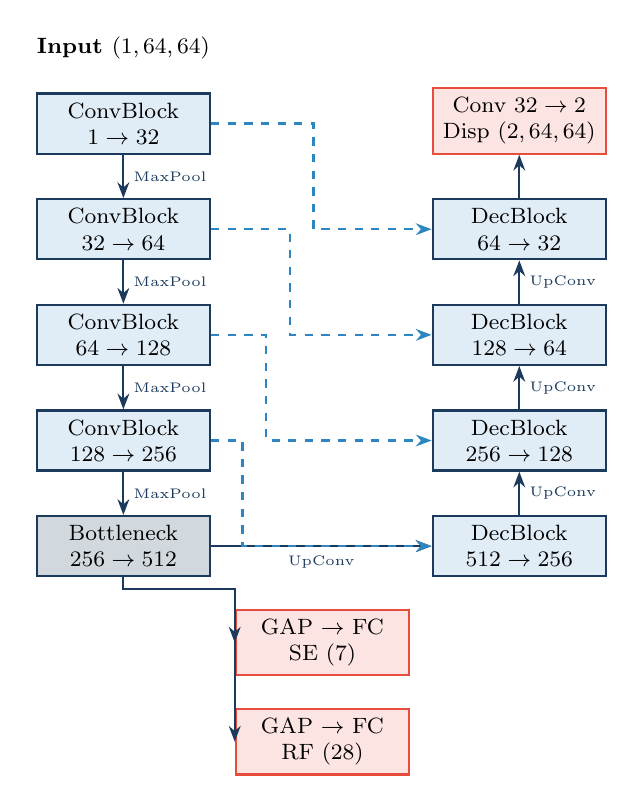
\begin{tikzpicture}[
    block/.style={rectangle, draw=darkblue, fill=accentblue!15, thick,
                  minimum width=2.2cm, minimum height=0.7cm, align=center,
                  font=\footnotesize},
    head/.style={rectangle, draw=highlightred, fill=highlightred!15, thick,
                 minimum width=2.2cm, minimum height=0.7cm, align=center,
                 font=\footnotesize},
    arr/.style={-{Stealth[length=2mm]}, thick, darkblue},
    skip/.style={-{Stealth[length=2mm]}, thick, accentblue, dashed},
    node distance=0.55cm
]
    % Encoder
    \node[block] (e1) {ConvBlock\\$1 \to 32$};
    \node[block, below=of e1] (e2) {ConvBlock\\$32 \to 64$};
    \node[block, below=of e2] (e3) {ConvBlock\\$64 \to 128$};
    \node[block, below=of e3] (e4) {ConvBlock\\$128 \to 256$};
    \node[block, below=of e4, fill=darkblue!20] (bn) {Bottleneck\\$256 \to 512$};

    % Arrows encoder
    \draw[arr] (e1) -- node[right, font=\tiny] {MaxPool} (e2);
    \draw[arr] (e2) -- node[right, font=\tiny] {MaxPool} (e3);
    \draw[arr] (e3) -- node[right, font=\tiny] {MaxPool} (e4);
    \draw[arr] (e4) -- node[right, font=\tiny] {MaxPool} (bn);

    % Decoder
    \node[block, right=2.8cm of bn] (d4) {DecBlock\\$512 \to 256$};
    \node[block, above=of d4] (d3) {DecBlock\\$256 \to 128$};
    \node[block, above=of d3] (d2) {DecBlock\\$128 \to 64$};
    \node[block, above=of d2] (d1) {DecBlock\\$64 \to 32$};
    \node[head, above=of d1] (dh) {Conv $32 \to 2$\\Disp $(2,64,64)$};

    % Arrows decoder
    \draw[arr] (bn) -- node[below, font=\tiny] {UpConv} (d4);
    \draw[arr] (d4) -- node[right, font=\tiny] {UpConv} (d3);
    \draw[arr] (d3) -- node[right, font=\tiny] {UpConv} (d2);
    \draw[arr] (d2) -- node[right, font=\tiny] {UpConv} (d1);
    \draw[arr] (d1) -- (dh);

    % Skip connections
    \draw[skip] (e4.east) -- ++(0.4,0) |- (d4.west);
    \draw[skip] (e3.east) -- ++(0.7,0) |- (d3.west);
    \draw[skip] (e2.east) -- ++(1.0,0) |- (d2.west);
    \draw[skip] (e1.east) -- ++(1.3,0) |- (d1.west);

    % Scalar heads
    \node[head, below right=0.4cm and 0.3cm of bn] (se) {GAP $\to$ FC\\SE $(7)$};
    \node[head, below=0.4cm of se] (rf) {GAP $\to$ FC\\RF $(28)$};
    \draw[arr] (bn.south) -- ++(0,-0.15) -| (se.west);
    \draw[arr] (bn.south) -- ++(0,-0.15) -| (rf.west);

    % Input label
    \node[above=0.3cm of e1, font=\footnotesize\bfseries] {Input $(1, 64, 64)$};
\end{tikzpicture}
\caption{Multi-Task U-Net architecture. Dashed arrows denote skip connections.
         GAP = Global Average Pooling, FC = Fully Connected layers.}
\label{fig:unet-arch}
\end{figure}

\subsection{ConvBlock}

Each \texttt{ConvBlock} consists of two consecutive convolution layers:
\[
    \text{Conv2d}(3{\times}3) \;\to\; \text{BN} \;\to\; \text{ReLU}
    \;\to\; \text{Conv2d}(3{\times}3) \;\to\; \text{BN} \;\to\; \text{ReLU}
\]
All convolutions use $\text{padding} = 1$ (preserving spatial dimensions) and
$\text{bias} = \text{False}$ (since batch normalization follows).

\subsection{Encoder}

The shared encoder has four stages with feature dimensions
$[32, 64, 128, 256]$. Each stage applies a \texttt{ConvBlock} followed by
$2 \times 2$ max-pooling, progressively reducing the spatial resolution:
\[
    64^2 \;\xrightarrow{\text{pool}}\; 32^2 \;\xrightarrow{\text{pool}}\;
    16^2 \;\xrightarrow{\text{pool}}\; 8^2 \;\xrightarrow{\text{pool}}\; 4^2.
\]
A bottleneck \texttt{ConvBlock} maps $256 \to 512$ channels at $4 \times 4$
spatial resolution.

\subsection{Displacement Decoder (Head 1)}

The decoder mirrors the encoder with four upsampling stages using transposed
convolutions (\texttt{ConvTranspose2d}, kernel $2$, stride $2$). At each level,
the upsampled features are concatenated with the corresponding encoder skip
connection and refined through a \texttt{ConvBlock}:
\[
    512 \;\to\; 256 \;\to\; 128 \;\to\; 64 \;\to\; 32.
\]
A final $1 \times 1$ convolution projects the 32-channel feature map to 2
channels, producing the displacement output $(B, 2, 64, 64)$.

\subsection{Strain Energy Head (Head 2)}

From the bottleneck representation $(B, 512, 4, 4)$:
\[
    \text{AdaptiveAvgPool}(1) \;\to\; \text{Flatten} \;\to\;
    \text{FC}(512, 128) \;\to\; \text{ReLU} \;\to\; \text{FC}(128, 7).
\]
Output: $(B, 7)$ -- strain energy at each of the seven displacement levels.

\subsection{Reaction Forces Head (Head 3)}

Identical structure to the strain energy head, with a different output dimension:
\[
    \text{AdaptiveAvgPool}(1) \;\to\; \text{Flatten} \;\to\;
    \text{FC}(512, 128) \;\to\; \text{ReLU} \;\to\; \text{FC}(128, 28).
\]
Output: $(B, 28)$ -- reaction forces (4 boundaries $\times$ 7 levels).


% ══════════════════════════════════════════════════════════════════════════════
\section{Model 2: Multi-Task Fourier Neural Operator}
\label{sec:fno}

\subsection{Architecture Overview}

The Multi-Task FNO learns solution operators in Fourier space through spectral
convolutions. It maintains \textbf{full spatial resolution} ($64 \times 64$)
throughout the network -- no pooling or upsampling is needed for the
displacement head. The total parameter count is approximately \textbf{2.7 million}.

\begin{figure}[H]
\centering
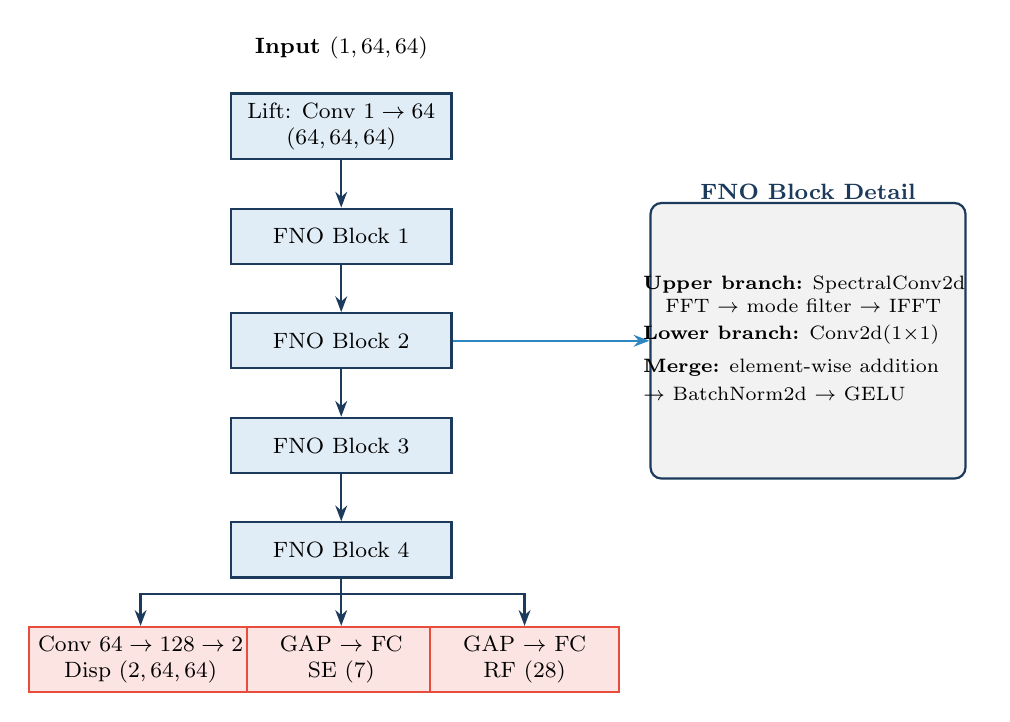
\begin{tikzpicture}[
    block/.style={rectangle, draw=darkblue, fill=accentblue!15, thick,
                  minimum width=2.8cm, minimum height=0.7cm, align=center,
                  font=\footnotesize},
    head/.style={rectangle, draw=highlightred, fill=highlightred!15, thick,
                 minimum width=2.4cm, minimum height=0.7cm, align=center,
                 font=\footnotesize},
    arr/.style={-{Stealth[length=2mm]}, thick, darkblue},
    node distance=0.6cm
]
    \node[block] (lift) {Lift: Conv $1 \to 64$\\$(64, 64, 64)$};
    \node[block, below=of lift] (f1) {FNO Block 1};
    \node[block, below=of f1] (f2) {FNO Block 2};
    \node[block, below=of f2] (f3) {FNO Block 3};
    \node[block, below=of f3] (f4) {FNO Block 4};

    \draw[arr] (lift) -- (f1);
    \draw[arr] (f1) -- (f2);
    \draw[arr] (f2) -- (f3);
    \draw[arr] (f3) -- (f4);

    % Heads
    \node[head, below left=0.6cm and -0.3cm of f4] (dh) {Conv $64 \to 128 \to 2$\\Disp $(2,64,64)$};
    \node[head, below=0.6cm of f4] (se) {GAP $\to$ FC\\SE $(7)$};
    \node[head, below right=0.6cm and -0.3cm of f4] (rf) {GAP $\to$ FC\\RF $(28)$};

    \draw[arr] (f4.south) -- ++(0,-0.2) -| (dh.north);
    \draw[arr] (f4) -- (se);
    \draw[arr] (f4.south) -- ++(0,-0.2) -| (rf.north);

    \node[above=0.3cm of lift, font=\footnotesize\bfseries] {Input $(1, 64, 64)$};

    % FNO Block detail
    \node[right=2.5cm of f2, draw=darkblue, thick, rounded corners,
          fill=lightgray, minimum width=4cm, minimum height=3.5cm] (detail) {};
    \node[above=-0.1cm of detail.north, font=\footnotesize\bfseries\color{darkblue}]
          {FNO Block Detail};

    \node[font=\scriptsize, align=left] at (detail.center) {%
        \begin{tabular}{@{}l@{}}
        \textbf{Upper branch:} SpectralConv2d\\
        \quad FFT $\to$ mode filter $\to$ IFFT\\[2pt]
        \textbf{Lower branch:} Conv2d($1{\times}1$)\\[4pt]
        \textbf{Merge:} element-wise addition\\[2pt]
        $\to$ BatchNorm2d $\to$ GELU
        \end{tabular}
    };

    \draw[arr, accentblue] (f2.east) -- (detail.west);
\end{tikzpicture}
\caption{Multi-Task FNO architecture with FNO block detail.}
\label{fig:fno-arch}
\end{figure}

\subsection{Spectral Convolution}

The core operation is the \textbf{SpectralConv2d} layer, which learns weights
directly in the Fourier domain:

\begin{enumerate}[leftmargin=2em]
    \item Apply 2D real FFT to the input: $\hat{x} = \text{rfft2}(x)$.
    \item Retain only the lowest $M_1 \times M_2$ Fourier modes (default:
          $M_1 = M_2 = 16$).
    \item Multiply selected modes with learnable complex weights via
          Einstein summation:
          \[
              \hat{y}_{b,o,k_1,k_2} = \sum_{i} \hat{x}_{b,i,k_1,k_2}
              \cdot W_{i,o,k_1,k_2}, \qquad W \in \mathbb{C}^{C_\text{in}
              \times C_\text{out} \times M_1 \times M_2}.
          \]
          Two weight tensors handle positive and negative frequency corners.
    \item Apply inverse FFT: $y = \text{irfft2}(\hat{y})$.
\end{enumerate}

Weights are initialized with scale $1 / (C_\text{in} \cdot C_\text{out})$.

\subsection{FNO Block}

Each FNO block combines spectral and pointwise convolution paths:
\[
    \text{out} = \text{GELU}\!\Big(\text{BN}\big(
        \underbrace{\text{SpectralConv2d}(x)}_{\text{global (Fourier)}}
        + \underbrace{\text{Conv2d}_{1 \times 1}(x)}_{\text{local (pointwise)}}
    \big)\Big).
\]
The spectral branch captures global spatial patterns through frequency-domain
filtering, while the pointwise branch processes channel interactions locally.
Four such blocks are stacked in sequence, all operating at full $64 \times 64$
resolution.

\subsection{Lifting and Projection}

\begin{itemize}[leftmargin=2em]
    \item \textbf{Lift}: A $1 \times 1$ convolution maps the single-channel
          input to $W = 64$ channels: $(B, 1, 64, 64) \to (B, 64, 64, 64)$.
    \item \textbf{Projection}: After the FNO layers, each head projects
          the latent features to its respective output.
\end{itemize}

\subsection{Output Heads}

\paragraph{Displacement Head.}
Two $1 \times 1$ convolutions with GELU activation:
\[
    \text{Conv}(64, 128) \;\to\; \text{GELU} \;\to\; \text{Conv}(128, 2).
\]
Output: $(B, 2, 64, 64)$.

\paragraph{Strain Energy Head.}
\[
    \text{AdaptiveAvgPool}(1) \;\to\; \text{Flatten} \;\to\;
    \text{FC}(64, 128) \;\to\; \text{ReLU} \;\to\; \text{FC}(128, 7).
\]
Output: $(B, 7)$.

\paragraph{Reaction Forces Head.}
\[
    \text{AdaptiveAvgPool}(1) \;\to\; \text{Flatten} \;\to\;
    \text{FC}(64, 128) \;\to\; \text{ReLU} \;\to\; \text{FC}(128, 28).
\]
Output: $(B, 28)$.


% ══════════════════════════════════════════════════════════════════════════════
\section{Training Process}
\label{sec:training}

Both models share an identical training pipeline, enabling fair comparison.

\subsection{Loss Function}

The total loss is an \textbf{unweighted sum} of MSE losses across the three
tasks:
\[
    \mathcal{L}_\text{total} = \underbrace{\frac{1}{N}
    \sum_{i} \| \hat{u}_i - u_i \|_2^2}_{\mathcal{L}_\text{disp}}
    + \underbrace{\frac{1}{N} \sum_{i} \| \hat{s}_i - s_i \|_2^2
    }_{\mathcal{L}_\text{SE}}
    + \underbrace{\frac{1}{N} \sum_{i} \| \hat{r}_i - r_i \|_2^2
    }_{\mathcal{L}_\text{RF}},
\]
where $N$ is the batch size, $\hat{\cdot}$ denotes predictions, and
$u$, $s$, $r$ are the displacement, strain energy, and reaction force targets,
respectively.

\subsection{Hyperparameters}

\begin{table}[H]
\centering
\caption{Training hyperparameters (shared by both models).}
\label{tab:hparams}
\begin{tabular}{@{}ll@{}}
\toprule
\textbf{Parameter} & \textbf{Value} \\
\midrule
Optimizer             & Adam \\
Learning rate         & $1 \times 10^{-3}$ \\
Weight decay          & $1 \times 10^{-5}$ \\
Batch size            & 64 \\
Maximum epochs        & 50 \\
LR scheduler          & ReduceLROnPlateau \\
\quad Reduction factor & 0.5 \\
\quad Scheduler patience & 3 epochs \\
Early stopping patience & 7 epochs \\
Random seed           & 42 \\
\bottomrule
\end{tabular}
\end{table}

\subsection{Learning Rate Schedule}

The learning rate is managed by \texttt{ReduceLROnPlateau}, which monitors
the total validation loss. When validation loss stops decreasing for 3
consecutive epochs, the learning rate is halved:
\[
    \text{lr}_\text{new} = 0.5 \times \text{lr}_\text{current}.
\]

\subsection{Early Stopping}

Training terminates early if the total validation loss does not improve for
7 consecutive epochs. The model checkpoint with the lowest validation loss is
saved as \texttt{best\_model.pt}.

\subsection{Training Algorithm}

\begin{algorithm}[H]
\caption{Multi-Task Training Loop}
\label{alg:training}
\begin{algorithmic}[1]
\Require Training set $\mathcal{D}_\text{train}$, validation set
         $\mathcal{D}_\text{val}$, model $f_\theta$
\State Initialize $\theta$, optimizer, scheduler
\State $\text{best\_loss} \gets \infty$, $\text{wait} \gets 0$
\For{epoch $= 1, \ldots, 50$}
    \For{each mini-batch $(X, u, s, r)$ in $\mathcal{D}_\text{train}$}
        \State $\hat{u}, \hat{s}, \hat{r} \gets f_\theta(X)$
        \State $\mathcal{L} \gets \text{MSE}(\hat{u}, u) + \text{MSE}(\hat{s}, s)
               + \text{MSE}(\hat{r}, r)$
        \State Backpropagate $\nabla_\theta \mathcal{L}$; update $\theta$
    \EndFor
    \State Compute $\mathcal{L}_\text{val}$ on $\mathcal{D}_\text{val}$
    \State Update scheduler with $\mathcal{L}_\text{val}$
    \If{$\mathcal{L}_\text{val} < \text{best\_loss}$}
        \State $\text{best\_loss} \gets \mathcal{L}_\text{val}$;
               save checkpoint; $\text{wait} \gets 0$
    \Else
        \State $\text{wait} \gets \text{wait} + 1$
    \EndIf
    \If{$\text{wait} \geq 7$}
        \State \textbf{break} \Comment{Early stopping}
    \EndIf
\EndFor
\end{algorithmic}
\end{algorithm}


% ══════════════════════════════════════════════════════════════════════════════
\section{Evaluation}
\label{sec:evaluation}

\subsection{Metrics}

Models are evaluated on the held-out test set using the following metrics
(computed after denormalization):

\begin{itemize}[leftmargin=2em]
    \item \textbf{Displacement -- Relative $L^2$ error}:
    \[
        e_\text{rel} = \frac{\| \hat{u} - u \|_2}{\| u \|_2}
    \]
    averaged over all test samples.

    \item \textbf{Displacement -- MSE}: Pixel-wise mean squared error over
          both channels.

    \item \textbf{Strain energy -- MSE}: Mean squared error averaged over the
          7-element vectors.

    \item \textbf{Reaction forces -- MSE}: Mean squared error averaged over
          the 28-element vectors.
\end{itemize}

\subsection{Denormalization}

Predictions are converted back to physical units before metric computation:
\[
    y = \hat{y} \cdot \sigma + \mu,
\]
where $\mu$ and $\sigma$ are the per-channel statistics stored during
preprocessing.


% ══════════════════════════════════════════════════════════════════════════════
\section{Model Comparison}
\label{sec:comparison}

\begin{table}[H]
\centering
\caption{Architectural comparison of the two surrogate models.}
\label{tab:comparison}
\begin{tabularx}{\textwidth}{@{}lXX@{}}
\toprule
\textbf{Aspect} & \textbf{Multi-Task U-Net} & \textbf{Multi-Task FNO} \\
\midrule
Backbone type &
    Local convolutions ($3 \times 3$) with pooling/upsampling &
    Spectral convolutions via FFT (global receptive field) \\[4pt]

Parameters &
    ${\sim}8.1$M &
    ${\sim}2.7$M \\[4pt]

Spatial resolution &
    Progressive downsampling ($64 \to 4$) then upsampling &
    Constant $64 \times 64$ throughout \\[4pt]

Receptive field &
    Local, grows with depth &
    Global from layer 1 (full spectrum) \\[4pt]

Skip connections &
    Yes (encoder $\to$ decoder at each level) &
    No \\[4pt]

Scalar head input &
    Bottleneck features ($512$ ch, $4 \times 4$) &
    Final FNO layer ($64$ ch, $64 \times 64$) \\[4pt]

Normalization &
    BatchNorm (after each conv) &
    BatchNorm (after spectral + pointwise sum) \\[4pt]

Activation &
    ReLU (throughout) &
    GELU (backbone) / ReLU (scalar heads) \\[4pt]

Decoder for displacement &
    Transposed convolutions with skip connections &
    Two $1 \times 1$ convolutions (no upsampling needed) \\
\bottomrule
\end{tabularx}
\end{table}

\subsection{Theoretical Considerations}

\begin{itemize}[leftmargin=2em]
    \item The \textbf{FNO} is theoretically well-suited for PDE surrogate
          modeling due to its ability to learn mappings between function spaces
          via spectral representations. Its global receptive field enables
          capturing long-range spatial correlations from the first layer.

    \item The \textbf{U-Net} benefits from well-established multi-scale
          feature extraction and skip connections that preserve fine-grained
          spatial details during reconstruction. Its inductive bias toward
          local features is effective for capturing material interfaces.

    \item The FNO uses ${\sim}3\times$ fewer parameters, making it more
          computationally efficient at inference time. However, the FFT
          operations introduce overhead that may offset parameter savings for
          small input sizes.
\end{itemize}


% ══════════════════════════════════════════════════════════════════════════════
\section{FNO-Specific Hyperparameters}
\label{sec:fno-hparams}

\begin{table}[H]
\centering
\caption{FNO-specific architecture hyperparameters.}
\begin{tabular}{@{}llp{7cm}@{}}
\toprule
\textbf{Parameter} & \textbf{Value} & \textbf{Description} \\
\midrule
Fourier modes ($M$) & 16 & Number of frequency modes retained per spatial
    dimension. Controls the frequency resolution of learned filters. \\[4pt]
Width ($W$) & 64 & Channel dimension throughout FNO layers. \\[4pt]
Number of layers & 4 & Number of stacked FNO blocks. \\[4pt]
Weight dtype & \texttt{cfloat} & Complex-valued learnable weights in Fourier
    space. \\
\bottomrule
\end{tabular}
\end{table}


% ══════════════════════════════════════════════════════════════════════════════
\section{Implementation Details}
\label{sec:implementation}

\subsection{Data Loading}

Both models use PyTorch's \texttt{DataLoader} with:
\begin{itemize}[leftmargin=2em]
    \item Memory-mapped NumPy arrays (\texttt{mmap\_mode="r"}) for efficient
          I/O on large datasets.
    \item Pinned memory (\texttt{pin\_memory=True}) for faster GPU transfers.
    \item 4 parallel data loading workers.
\end{itemize}

\subsection{Checkpoint Format}

The saved checkpoint (\texttt{best\_model.pt}) contains:
\begin{itemize}[leftmargin=2em]
    \item \texttt{model\_state\_dict} -- Trained model weights.
    \item \texttt{optimizer\_state\_dict} -- Optimizer state for resuming.
    \item \texttt{epoch} -- Epoch number of the best checkpoint.
    \item \texttt{val\_loss} -- Per-task validation losses at checkpoint.
    \item \texttt{train\_loss} -- Per-task training losses at checkpoint.
    \item \texttt{hparams} -- Architecture hyperparameters (FNO only).
\end{itemize}

\subsection{Inference Pipeline}

For prediction on new images:
\begin{enumerate}[leftmargin=2em]
    \item Load image (supports \texttt{.txt}, \texttt{.jpeg}, \texttt{.png}).
    \item Binarize if needed (threshold at 0.5 for grayscale images).
    \item Downsample to $64 \times 64$ via center crop + block averaging.
    \item Normalize and run forward pass.
    \item Denormalize outputs to physical units.
    \item Generate FEA-style visualization with displacement heatmaps,
          strain energy curves, and reaction force plots.
\end{enumerate}

\end{document}
